\documentclass[journal]{IEEEtran}
% IEEE Transactions on Industrial Informatics -- anonymous regular-paper draft
% Compile: latexmk -pdf main.tex
\usepackage{amsmath,amssymb,amsfonts}
\usepackage{algpseudocode}
% Local XeTeX/Tectonic builds: route IEEEtran's ptm (Times) family requests to
% the legacy Times Type1 faces so metrics match the pdfLaTeX reference build;
% the latexmk -pdf (pdfLaTeX) path is unaffected.
\usepackage{iftex}
\ifxetex
  \DeclareFontFamily{TU}{ptm}{}
  \DeclareFontShape{TU}{ptm}{m}{n}{<->ptmr8t}{}
  \DeclareFontShape{TU}{ptm}{b}{n}{<->ptmb8t}{}
  \DeclareFontShape{TU}{ptm}{m}{it}{<->ptmri8t}{}
  \DeclareFontShape{TU}{ptm}{b}{it}{<->ptmbi8t}{}
  \DeclareFontShape{TU}{ptm}{m}{sl}{<->ptmro8t}{}
  \DeclareFontShape{TU}{ptm}{m}{sc}{<->ptmr8t}{}
\fi
\usepackage{graphicx}
\usepackage{booktabs}
\usepackage{tabularx}
\usepackage{array}
\usepackage[table]{xcolor}
\usepackage{stfloats}
\usepackage{placeins}
\usepackage{url}
\usepackage{balance}
\usepackage{etoolbox}
\urlstyle{same}
% Cross-references and citations. The cite package renders IEEE-style citation
% groups ([14]--[16], [20], [21]) with hyperref support.
\usepackage{cite}
\usepackage[colorlinks=true,linkcolor=black,citecolor=black,urlcolor=black]{hyperref}
\hypersetup{bookmarksnumbered=true,
  pdftitle={AgentWorkShop: A Modular Task-to-Device Integration Framework for Industrial Agents},
  pdfauthor={},
  pdfsubject={IEEE Transactions on Industrial Informatics},
  pdfkeywords={industrial agents, industrial communication, industrial informatics, production systems, semantic data integration}}

% Float placement only; IEEEtran margins and body type remain unchanged.
\setcounter{topnumber}{4}
\setcounter{bottomnumber}{3}
\setcounter{totalnumber}{7}
\setcounter{dbltopnumber}{2}
\renewcommand{\topfraction}{0.95}
\renewcommand{\bottomfraction}{0.80}
\renewcommand{\textfraction}{0.03}
\renewcommand{\floatpagefraction}{0.72}
\renewcommand{\dbltopfraction}{0.95}
\renewcommand{\dblfloatpagefraction}{0.72}

% Tight but conventional float separation; body type and margins are unchanged.
\setlength{\textfloatsep}{8pt plus 2pt minus 3pt}
\setlength{\dbltextfloatsep}{8pt plus 2pt minus 3pt}
\setlength{\intextsep}{7pt plus 2pt minus 3pt}
\setlength{\abovecaptionskip}{3pt plus 1pt minus 1pt}
\setlength{\belowcaptionskip}{2pt plus 1pt minus 1pt}

\newcommand{\system}{the platform}
% Review copy is anonymous. The AI-use statement is maintained in
% AI-DISCLOSURE.md for the journal-approved disclosure channel and is not
% compiled into this manuscript.
\newif\ifblindreview
\blindreviewtrue

\begin{document}
\bstctlcite{IEEEbstctl}

\title{AgentWorkShop: A Modular Task-to-Device Integration Framework for Industrial Agents}

\author{}
\markboth{IEEE Transactions on Industrial Informatics, Submitted Manuscript}{AgentWorkShop: Task-to-Device Integration}

\maketitle

\begin{abstract}
Industrial agents must translate task goals into device operations while
respecting changing production context and scene-specific signals and limits.
We present AgentWorkShop, an integration framework that connects task and
direct-operation entries to shared dispatch, maps semantic controls to device
drivers, and retains command receipts separately from subsequent observations.
Simulator checks examine protocol and node access, and two entry paths are
tested for their retained records. In a separate mock-driver test with
simulated approval decisions, every injected stale production context was
rejected before a write; removing the context comparison allowed six product
or run changes. Four deterministic simulator missions recorded on September
28, 2026, trace control requests and observations for injection molding, film
production, annealing, and wastewater treatment. In one trajectory per scene,
each reported final primary value fell within its target band. The tested
routes retained entry-specific records, and the missions reached their reported
target bands in simulation. The missions do not use a
language model to select setpoints; they do not establish human-review
effectiveness, statistical repeatability, or physical-plant performance, and
some secondary terminal measurements were not archived.
\end{abstract}

\begin{IEEEkeywords}
Industrial agents, industrial communication, industrial informatics,
production systems, semantic data integration.
\end{IEEEkeywords}

\IEEEpeerreviewmaketitle

\section{Introduction}
\IEEEPARstart{I}{ndustrial-agent} deployments translate task-level goals into
operations over production signals and equipment. A line-speed adjustment,
for example, depends on the active product, recipe, run, applicable limits,
and the control node mapped to the line. If that context changes while a
proposal is awaiting approval, a formerly admissible request may no longer be
appropriate. Device access also needs evidence at two distinct points: what
the command interface reported and what the process was later observed to do.
Connecting these steps across task and device interfaces is therefore a
central industrial integration problem.

Recent work explores end-to-end automation, control-sequence generation,
modular factory skills, and robotic-line control
\cite{xia2025control,huang2026made,koehle2026llmdriven,waseem2026pretrained}.
Other studies address programmable logic controller (PLC) code generation,
context-aware control, resource discovery, shop-floor coordination,
digital-twin fault handling, and natural-language machine access
\cite{liu2026agents4plc,wu2025instructmpc,lim2025llmenabled,zhao2026shopfloor,gill2025llmdt,hofmann2025nlc}.
Recent platforms further connect proposals to Asset Administration Shell
(AAS) models and signed approval, validate actions against process and
instrumentation diagrams (P\&IDs), or organize sensor--manufacturing
execution system (MES)--enterprise resource planning (ERP) evidence streams
\cite{graul2026aas,schall2026safe,lin2026agentic}. Together, these efforts
provide valuable methods for agent reasoning, production context, and
operation constraints.

These studies address complementary aspects of agent operation and motivate a
further integration question: how can different task engines and direct calls
use a common operation boundary while accounting for scene-specific devices,
production context, and route-specific evidence? AgentWorkShop provides such
a design. Registered harnesses connect agent engines to task context, while
direct representational state transfer (REST) calls reach the same
named-operation dispatcher. Scene blueprints map semantic signals to configured
drivers and provide targets and guards. The scope of the present experiments
does not establish that this design is unique or that all entry paths are
equivalent.

Fig.~\ref{fig:control-path} summarizes this control path. Task goals and
production context inform an operation proposal. Shared checks, route guards,
approval when required, and a pre-dispatch context recheck precede writes
through the device write-control (DCW) subsystem. Command receipts and
subsequent data-acquisition (DAQ) observations remain distinct records: a
readback can verify a setpoint, while a later observation describes the
measured process state without, by itself, establishing causation.

\begin{figure}[!b]
\centering
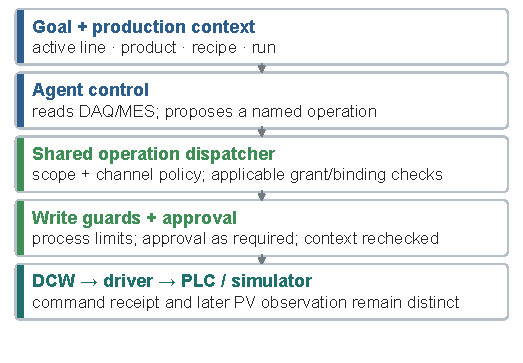
\includegraphics[width=\columnwidth]{resources/fig-agent-control.pdf}
\caption{Agent-control path for a configured industrial task. The agent uses
DAQ and MES context, passes shared operation checks, and routes writes through
process guards, conditional approval, and a pre-dispatch context recheck. DCW
and configured drivers provide device access; command receipts and later
process observations remain separate. Scene configuration supplies targets
and guards, while the application provides its optimization policy.}
\label{fig:control-path}
\end{figure}

AgentWorkShop implements this path as a modular task-to-device framework.
Task requests enter a collaboration runtime whose harness adapters connect
agent engines to production context and available operations. Direct calls
enter the operation dispatcher without creating a task. Scene blueprints and
channel profiles define the signals, objectives, guards, tools, and agent
bindings for a deployment. Fig.~\ref{fig:arch} shows these architectural
relationships, and Fig.~\ref{fig:runtime} follows one registered task through
the execution path.

This paper contributes a modular task-to-device integration design that
combines a shared dispatch boundary, scene-specific signal mappings, and
separate command and observation records. It also examines selected parts of
that design through complementary tests: simulator protocol and node access,
entry-specific records, stale approval-context rejection with a mock driver, and four process
missions. In the component test, every single-field context change was
refused before mock writes; this result concerns the tested approval check,
not human review. The missions trace requests and observations for part
weight, film thickness, strip hardness, and dissolved oxygen. Each scene has
one deterministic trajectory, and no language model selects its setpoints.
The checks do not establish equivalence between entry paths, comparative
performance, or physical-plant performance.

Section~II reviews related work. Section~III presents the architecture and
execution flow. Section~IV explains the cooperating modules and their device
access and evidence mechanisms. Section~V describes the simulation protocol
and results; Sections~VI and~VII discuss their implications and conclude.

\section{Related Work}
\label{sec:related}
This section positions the integration problem against plant-facing agents
and industrial abstractions for context, device operations, and operational
evidence. Table~\ref{tab:nearest} summarizes selected studies' reported
mechanisms and evaluation settings; it is not a matched performance
comparison or an exhaustive account of their implementations.

\subsection{Industrial Agents and Plant Integration}
Industrial-agent systems span end-to-end automation control, supervisory
services, programmable logic controller (PLC) interfaces, manufacturing
coordination, and operator-facing machine access. Xia et al. present a large
language model (LLM) framework for end-to-end automation
control \cite{xia2025control}; Huang et al. focus on automated control
generation for industrial cyber-physical systems \cite{huang2026made};
Biskupovic et al. study agent-based supervision
\cite{biskupovic2025supervision}; and Agents4PLC and InstructMPC address PLC
code generation and human--LLM control
\cite{liu2026agents4plc,wu2025instructmpc}. Manufacturing studies consider
resource-capability exploration \cite{lim2025llmenabled}, shop-floor
coordination \cite{zhao2026shopfloor}, and digital-twin fault handling
\cite{gill2025llmdt}. Natural-language machine access \cite{hofmann2025nlc}
and real-time LLM control of a robot-operated line
\cite{waseem2026pretrained} extend this work to operator interfaces and
robotic-line control.

Xia et al. connect cognitive, digital-twin, and physical-automation layers and
organize twin information as state snapshots, event messages, and plan
sequences \cite{xia2025architecture}. Other nearby designs expose factory-module
operations through the Model Context Protocol (MCP) with state-based tool
filtering, constrain
manufacturing plans, or compose semantic recipes from OPC Unified Architecture
(OPC UA) skills
\cite{koehle2026llmdriven,silva2025mcpmanufacturing,koehle2025semanticrecipes}.
Several recent systems also combine agent execution with approval, industrial
data, or audit records. Graul et al. ground proposals in the Asset
Administration Shell (AAS) and route approved actions through OPC UA Methods,
with signed approvals and audit logging \cite{graul2026aas}. Schall separates
advisory language-model agents from process and instrumentation diagram
(P\&ID)-grounded verification and execution, and evaluates structural checks
across five simulated process scenarios \cite{schall2026safe}; its context
includes supervisory control and data acquisition (SCADA) and standard
operating procedure (SOP) information. Lin and Chen build a governed
sensor--MES--ERP digital thread for closed-loop monitoring and control on real
manufacturing records \cite{lin2026agentic}. These designs address different
parts of the integration problem: asset-grounded approval, action validation,
and the organization of industrial evidence. The present paper describes a
complementary task-to-device path in which registered tasks and direct calls
reach named operation handlers and route-specific records remain with their
owning services. The cited studies' reported descriptions do not permit a
matched comparison of that entry-path arrangement; Table~\ref{tab:nearest}
therefore presents their mechanisms and evaluation contexts rather than
inferring missing capabilities.
\begin{table*}[!t]
\centering
\caption{Reported operation mechanisms and evaluations in selected
plant-facing studies. Evaluation settings and outcomes are source-specific;
this table does not compare performance across studies.}
\label{tab:nearest}
\small
\setlength{\tabcolsep}{3pt}
\begin{tabularx}{\textwidth}{@{}>{\raggedright\arraybackslash}p{1.8cm}>{\raggedright\arraybackslash}p{7.0cm}>{\raggedright\arraybackslash}X@{}}
\toprule
System & Reported operation and evidence structure & Reported evaluation \\
\midrule
Xia et al. \cite{xia2025architecture} & Cognitive, twin, and physical layers; twin snapshots, event messages, and plan sequences & Robotic automation and process-simulation cases \\
K{\"o}hle et al. \cite{koehle2026llmdriven} & Injected live state and state-based filtering; MCP-to-OPC UA operations and Message Queuing Telemetry Transport (MQTT) coordination & Nine simulated production challenges \\
Vieira da Silva et al. \cite{silva2025mcpmanufacturing} & Constrained multi-step plans over MCP manufacturing functions & Laboratory multi-step process \\
K{\"o}hle et al. \cite{koehle2025semanticrecipes} & Semantic recipes composed from OPC UA skills; virtual commissioning & Unity assembly-workstation proof of concept \\
Graul et al. \cite{graul2026aas} & AAS-grounded proposals, signed human approval, PLC-validated OPC UA Methods, and immutable audit log & Two laboratory PoCs; single scripted runs \\
Schall \cite{schall2026safe} & P\&ID-, SCADA-, and SOP-grounded proposal verification with gated execution & Five simulated scenarios; 43 proposals and 50 LLM runs \\
Lin and Chen \cite{lin2026agentic} & Governed sensor--MES--ERP digital thread with SOP-, risk-, and capability-aware action gating & 25,275 real records; operational metrics \\
\midrule
This work & Shared dispatcher and scene-bound DAQ/DCW nodes; separate command and subsequent observation records & Simulator protocol and onboarding checks; mock approval-context test; four deterministic missions \\
\bottomrule
\end{tabularx}
\end{table*}

The operation checks complement safety-aware decision support
\cite{jiang2026agentic} and operate alongside the plant's configured process
protection.

\subsection{Production Context, Agent Interfaces, and Automation}
Industrial integration also depends on abstractions that are not specific to
agent architectures. The Model Context Protocol (MCP) specifies interoperable
tool discovery and call mechanisms \cite{mcp2024}; the operation-level scope,
policy, grant, and binding checks discussed here are AgentWorkShop's own
dispatcher rules, distinct from MCP transport authorization. In parallel,
ISA-88 and ISA-95 describe recipes and production operations
\cite{isa88_2010,isa95_2025}. Run-to-run methods connect process observations
to successive production runs \cite{moyne2000r2r}. Human--automation research
also formalizes the allocation of information acquisition, analysis, decisions,
and actions between people and automation \cite{parasuraman2000model}. At the
agent level, AgentSpec and CaMeL address tool behavior and capability-based
information flow \cite{wang2025agentspec,debenedetti2025camel}. Together, these standards
and agent-level mechanisms provide abstractions for production context, tool
interaction, and information flow. AgentWorkShop brings these abstractions into
one execution path: task and direct-operation calls converge on named handlers,
scene mappings connect semantic controls to configured drivers, and owning
services retain command receipts and process observations. Section~V examines
simulated node access, mock approval-context checks, and operation--response
sequences in four simulated process scenes. The deterministic missions do not
test every entry route or establish the effectiveness of human approval.

\section{System Design}
\label{sec:design}
AgentWorkShop is designed for industrial tasks whose agents, production
contexts, interfaces, and process signals vary between deployments. Its
architecture organizes these variations around shared task and operation
services, checks each proposed operation against the active production
context before device routing, and retains route-specific evidence that
distinguishes a command receipt from a measured process response.

\begin{figure*}[!t]
\centering
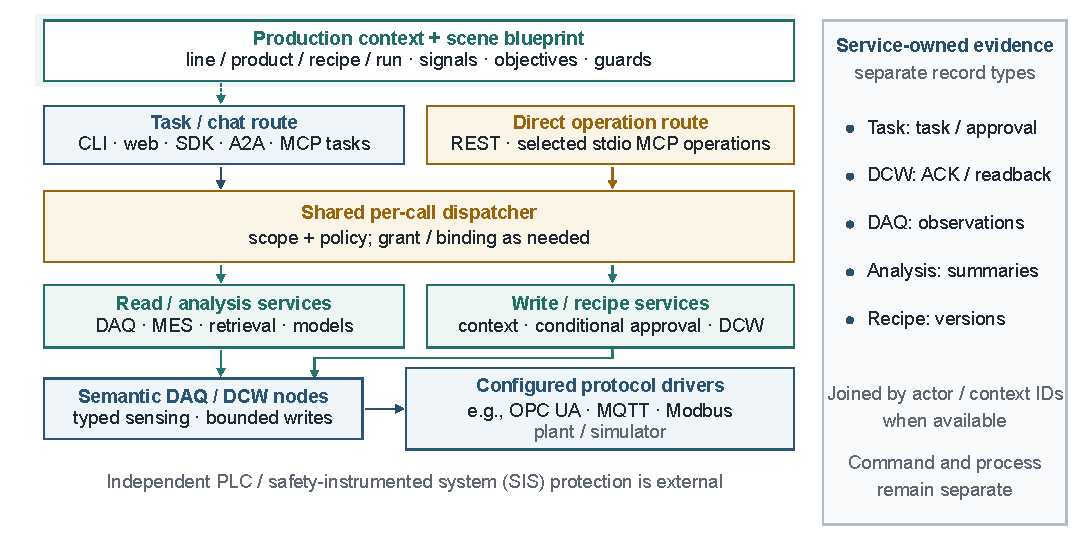
\includegraphics[width=\textwidth]{resources/fig-architecture-2026-9pt.pdf}
\caption{Architecture and record ownership. Task/chat routes enter the
collaboration runtime; direct REST and stdio-MCP calls enter shared dispatch
checks without creating a task. One dashed link marks configuration. Write
routes apply interval admission and, when configured, approval; recipe dispatch omits the
previous-recipe window. The shared dispatcher always
checks scope and channel policy, with grant and resource-binding checks applied
when required by the operation. Owning services retain distinct records; plant
controllers and safety systems retain equipment interlocks.}
\label{fig:arch}
\end{figure*}

\subsection{Design Rationale and Requirements}
\label{sec:principles}
Five requirements---scene variability, harness variability, operation
authority, outcome observability, and extensibility---shape the design.
Scene variability is represented by blueprints and semantic driver mappings;
harness variability by registered adapters; operation authority by shared
dispatch checks and route-specific guards and admission; outcome observability
by service-owned task, receipt, and observation records; and extensibility by
registered interfaces for agent engines and device drivers. Tool visibility
is separate from write authorization, and actuator writes converge on the
shared DCW admission point.

A scene blueprint bundles the process preset, signal inventory, DAQ/DCW driver
mappings, and target and guard rules; judged operation records and later
observations remain distinct evidence.

During setup, the integrator binds a validated blueprint to the active
line--product--recipe--run tuple, maps semantic nodes to drivers, and declares
target bands and guards. At runtime, the dispatcher checks current authority
before the handler issues a command; the handler returns a receipt, and DAQ
records subsequent observations.

\subsection{Layered Architecture}
\label{sec:layers}
\label{sec:arch}
Fig.~\ref{fig:arch} summarizes the access routes, shared dispatch path,
production services, semantic I/O, configured drivers, and service ownership
of records. Task and chat routes enter the
collaboration band, which contains workspaces, channels, task queues, shared
memory, mailboxes, task templates, and harness adapters. A \emph{task route}
is an execution path through this runtime; a \emph{harness adapter} connects
an agent engine to its task execution interface. Direct REST tool
calls and the stdio MCP operation bridge bypass task execution in that band
(the upper-right direct-operation entry in
Fig.~\ref{fig:arch}) and enter the shared governance block without creating a
task or starting a harness turn; MCP management and task methods remain on
their service routes. Direct calls resolve current route state at invocation,
without an agent-turn prompt or a task record.
The governance block projects the operation catalog and applies the per-call
checks. Write handlers apply admission limits and request approval when the
operation and its configuration require it. The
context block supplies the active line--product--recipe--run tuple to the gate
and scene maps, objectives, and guards to the handlers. The dashed link from
that block in Fig.~\ref{fig:arch} marks this configuration relationship; the
runtime assembles prompt-time context from the same records. The service band,
behind a route-handler interface that selects an adapter, provides
acquisition, write control, analysis, retrieval, and optional model services.
Field I/O resolves semantic nodes to built-in or plugin drivers for a plant or
simulator.

Each band has a distinct responsibility: task/chat routes enter the runtime,
direct operations enter the dispatcher, and both use shared checks. Harness
adapters supply agent-specific interaction, semantic nodes hide protocol
details, and the driver registry provides the device-facing extension point.
Owning services retain task, command, observation, and configuration records
separately and link them to actor and production context.

\subsection{Cross-Module Execution Flow}
\label{sec:executionflow}
Fig.~\ref{fig:runtime} summarizes a task turn from entry through operation
execution, with route-specific evidence retained by owning services. Registered
harness adapters receive a scoped tool catalog during setup and supported
registry refreshes; the runtime assembles prompt-time production context from
current records for each agent turn. For each returned tool call, the shared dispatcher rechecks
invocation scope and channel policy and, for industrial operations, current
grant and binding conditions before handler selection. The selected handler
then applies route-specific guards, active-run checks, approval
revalidation, and device-I/O steps as applicable. Command receipts and later
process observations remain distinct records.

For an industrial operation $u$ by agent $a$ in channel $c$, define the
shared dispatch condition as
\begin{equation}
\mathcal{A}(a,c,u)=\bigwedge_{X\in\mathcal{C}(u)}X(a,c,u),
\label{eq:dispatch-contract}
\end{equation}
where $S$, $P$, $G$, and $B$ denote invocation scope, current channel policy,
runtime grant, and the agent's binding to referenced resources, respectively.
$\mathcal{C}(u)\subseteq\{S,P,G,B\}$ is the set of predicates declared for
operation $u$; it always contains $S$ and $P$. The grant predicate $G$ is
omitted only for an explicitly grant-exempt industrial tool, and $B$ is
included when the operation declares resource references. A declared
no-reference operation omits $B$. Each included check must pass before
handler selection. The policy predicate includes channel tool selection,
profile, and duty-separation checks where configured. Once these predicates
pass, the selected route applies its guards and any required approval, then rechecks
authority, context, and applicable limits before device dispatch.

For direct REST invocation, the service establishes $a$ and $c$ before applying
these checks: an agent token must match the requested agent identifier, or an
authenticated user must be the channel owner or an administrator. The manager
loads the channel-agent record and rechecks scope and policy; industrial
operations then pass the shared grant and binding checks. Handlers resolve live
production state from request identifiers and owning services.

Fig.~\ref{fig:execution} gives reference pseudocode summarizing the
registered-harness task path. Direct REST tool invocation
bypasses the task runtime and harness but enters the same shared dispatcher.
Route-specific timing, approval, and evidence rules are detailed in
Section~\ref{sec:modules}.

\begin{figure*}[!t]
\centering
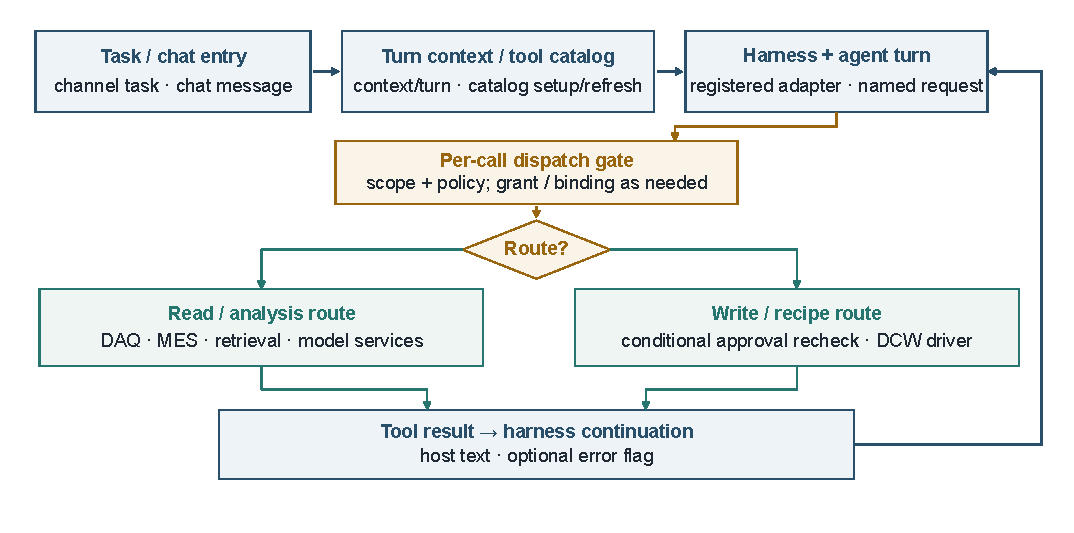
\includegraphics[width=\textwidth]{resources/fig-runtime-2026-9pt.pdf}
\caption{Registered-harness task flow. The runtime invokes the adapter with a
scoped catalog. Scope and channel policy are checked for every call; grant
applies to non-exempt industrial operations, and binding applies when resource
references are declared (figure label: scope + policy; grant / binding as needed). Failed
checks return tool errors. The read path
retrieves data. The write path applies route guards, conditional approval and
its context revalidation, DCW admission, and receipt grading; a later process observation
is separate. Results return to the harness. Device-level interlocks remain
with the configured plant-control layer.}
\label{fig:runtime}
\end{figure*}

\begin{figure}[!t]
\centering
\begin{algorithmic}[1]
\Require task $q$, channel $c$, bound agent $a$, registered scoped catalog $T$
\Ensure task result; any retained evidence remains with its owning service
\State $x_t \gets \Call{ResolvePromptContext}{c,q}$
\State $m \gets \Call{RetrieveMemory}{q}$
\State $p \gets \Call{AssemblePrompt}{q,x_t,m}$
\State $h \gets \Call{InvokeRegisteredHarness}{a,p,T}$
\ForAll{tool request $u$ returned by $h$}
  \State $g \gets \Call{CheckScopeAndChannelPolicy}{a,c,u}$
  \If{\textbf{not} $g$}
    \State \Call{EmitToolErrorToHarness}{h,u}; \textbf{continue}
  \EndIf
  \If{$u$ is an industrial operation}
    \State $v \gets \Call{CheckApplicableGrantBinding}{a,u}$
    \If{\textbf{not} $v$}
      \State \Call{EmitToolErrorToHarness}{h,u}
      \State \textbf{continue}
    \EndIf
  \EndIf
  \State $k \gets \Call{SelectHandler}{u}$
  \State $r \gets \Call{ExecuteRouteHandler}{k,a,c,u}$
  \Comment{handler resolves live state and may persist route-specific records}
  \State \Call{EmitDeclaredToolResultToHarness}{h,r}
\EndFor
\State \Return task state and tool results
\end{algorithmic}
\caption{Reference pseudocode for the registered-harness task path. Direct
operation calls use the shared dispatcher from their own entry point. Each
route persists its records through the owning service and returns its declared
response to the harness.}
\label{fig:execution}
\end{figure}

\section{Module Functions and Integration}
\label{sec:modules}
The architecture in Section~\ref{sec:design} assembles task context,
dispatches operations, and connects device access to separate records of
commands and observations. The following subsections explain the handoffs
between these functions.

\subsection{Task, Harness, and Context}
Task and chat entry points create or join a workspace channel. The task
runtime manages membership, task state, and shared execution context; a
harness registry adapts each supported agent engine to a common execution
interface. At each agent turn, the prompt builder assembles the task, active
scene description, production context, channel profile, agent binding, and
retrieved memory. This keeps engine-specific interaction behind the harness
interface while preserving the current line and operation context for the
agent.

Direct REST and selected stdio-MCP operation calls reach the same dispatcher
without a task or harness turn. REST authentication and identity resolution
follow Section~\ref{sec:executionflow}; each handler reads live route state
at invocation. Handlers receive the resolved actor, channel, and operation
arguments through the same interface for either entry route; records are keyed
by the identifiers supplied in each request. A registered task additionally
receives prompt context and a scoped tool catalog. Catalog visibility alone
does not grant write authority: the dispatcher checks authority at invocation.

\subsection{Shared Dispatch and Device Admission}
\label{sec:governed}
The dispatcher is the shared operation boundary. As specified by
(\ref{eq:dispatch-contract}), it checks invocation scope and channel policy
for every call; grant is skipped only for a grant-exempt industrial tool,
and binding applies when the operation declares resource references.
Applicable checks precede handler selection. Handlers revalidate route-specific state at
execution time, using the current policy and grant for each invocation.
Scene blueprints define device and signal maps, objectives, and process
guards. Capability profiles and tool policies narrow available operations,
while bindings constrain accessible nodes, controls, and recipes. Optional
DAQ, MES, analysis, retrieval, optimization, and digital-twin services are
invoked through registered handlers. The application supplies its optimization
strategy while the framework coordinates operation execution.

Actuator writes converge on the shared DCW admission point.
For an online node write, the admissible value interval is
\begin{equation}
\mathcal{I}^{\mathrm{online}}_n(t)=
\mathcal{H}_n\cap\mathcal{B}_n\cap\mathcal{P}_n(t)\cap\mathcal{R}_n(t),
\label{eq:admission}
\end{equation}
where $\mathcal{H}_n$ is the hard engineering range and
$\mathcal{B}_n$, $\mathcal{P}_n$, and $\mathcal{R}_n$ are the baseline,
active-product, and active-recipe limits; the subscripted limits here are
distinct from the policy and binding predicates of
(\ref{eq:dispatch-contract}). Missing optional limits impose no
restriction; an empty intersection rejects the request and identifies the
excluding layer. Recipe dispatch validates the replacement recipe against
the hard, baseline, and product limits rather than the previous recipe
window. Step, interval, and hold-window checks also constrain each route.
These software checks bound commands alongside independent
programmable-logic-controller and safety-instrumented protection.

\subsection{Approval, Execution, and Evidence}
\label{sec:routes}
\label{sec:mech}
\label{sec:objective}
\label{sec:nodeexec}
\label{sec:ack}
\label{sec:agentloop}
Routes add timing checks and, when required by operation and configuration,
approval checks. Online
node writes enforce a 60\,s minimum spacing; recipe trials use a per-line
cadence (300\,s by default), and recipe intervals are anchored to approval.
Manual approval binds an actor and proposed operation to candidate values,
applicable limits, expiry, and the active line--product--recipe--run tuple.
After approval, the handler rechecks authority and compares the current tuple
with the approved tuple before entering DCW dispatch. Single-parameter waits
expire after 180\,s by default; recipe-dispatch approvals use a 30-minute
window. A changed recipe definition requires a new
\texttt{recipe\_apply} proposal.

Fig.~\ref{fig:hitl}(a) illustrates the four-layer value interval in
Eq.~(\ref{eq:admission}) using an illustrative rotational-speed
configuration in revolutions per minute (rpm). Panel (b)
shows a symbolic approval followed by authority and context rechecks; its
values illustrate the approval sequence.

\begin{figure*}[!t]
\centering
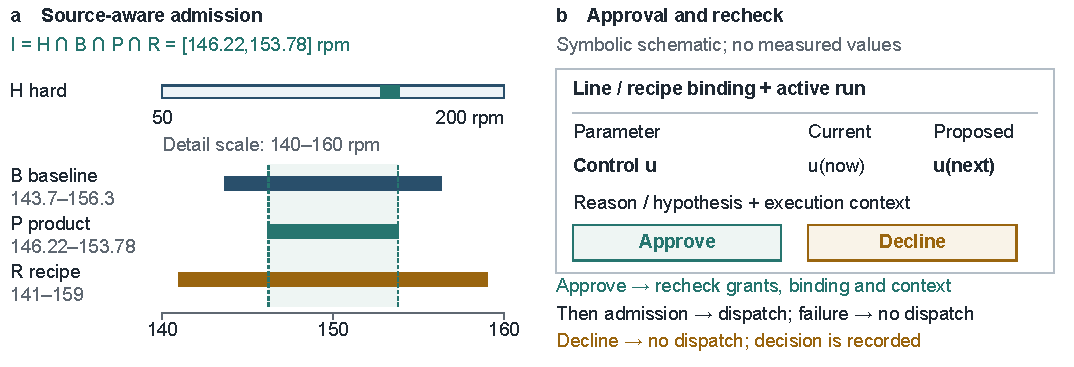
\includegraphics[width=\textwidth]{resources/fig-admission-hitl-2026.pdf}
\caption{Admission and approval boundaries. (a) An illustrative rotational-speed
configuration in revolutions per minute (rpm): online node interventions use the
four-layer interval of Eq.~(\ref{eq:admission}), whereas recipe dispatch
omits the previous recipe window. (b) Symbolic human approval binds a
proposed action and its context tuple; execution rechecks the active
line--product--recipe--run context, authority, and applicable limits before
device dispatch.}
\label{fig:hitl}
\end{figure*}

A \texttt{recipe\_trial} illustrates the operation sequence: the handler
checks the bound recipe, active run, candidate parameters, and route timing;
if required, it requests approval; after revalidation, it submits a bounded
batch through the configured driver and returns a per-parameter receipt.
The caller obtains later DAQ observations separately and may then update,
apply, or roll back a recipe. A trial neither saves nor applies a recipe
version. The driver registry maps semantic controls to configured protocol
drivers, keeping protocol details out of agent operation arguments.

For a concrete illustration, consider a simulated coating line whose semantic
line-speed control is mapped to a Modbus TCP write node. A request to change
the setpoint from 37 to 39\,m/min is inside a 28--48\,m/min recipe window;
the remaining applicable limits and timing checks must also pass. If the
configured policy requires approval, the proposal binds the candidate and
active production context, and the handler rechecks that context before
dispatch. The driver then returns a graded receipt. A later acquisition sample
is stored separately and can be associated with the operation when the route
provides the necessary context and timestamps. This example illustrates the
handoffs, not a recorded human decision or a particular process response; the
simulator onboarding replay in Section~\ref{sec:eval} used test-only automatic
approval.

Receipts and observations answer different questions. A command result is
graded as readback-verified, transport-acknowledged, or unverified; a
readback mismatch can trigger up to three reads at 2\,s intervals. Recipe
batches retain per-parameter verification outcomes. A readback-verified result
records that the returned value matched the request; a transport acknowledgement
alone does not establish that the device applied it, and an unverified result
does not establish a matching readback. DAQ stores subsequent timestamped
process observations, while recipe history, approvals, and task records remain
with their owning services. Identifiers and timestamps can link these records
when available, but a later observation alone does not prove that the command
caused the measured change. Section~\ref{sec:eval} evaluates selected parts of
this evidence chain under the stated test conditions.


\section{Experimental Evaluation}
\label{sec:eval}
The evaluation examines configured protocol and node access, entry-specific
records, approval-context checks, and control requests and observations during
optimization. Protocol connectivity and
four optimization missions were recorded on September 28, 2026. The missions
cover injection molding, biaxially oriented polyethylene terephthalate
(BOPET) film production, continuous annealing, and anaerobic/anoxic/oxic
wastewater treatment. A separate later onboarding replay and mock-state
approval test and two entry-path checks examine separate integration mechanisms;
they are not additional trials of the four missions. Table~\ref{tab:missions}
summarizes the process values, and Fig.~\ref{fig:missions} shows the recorded
intermediate observations.

\subsection{Test Design and Interpretation}
\label{sec:eval-protocol}
The missions ran against locally configured process simulators, using a
deterministic scenario-specific control routine and a fixed random seed.
The routines inspected process values and requested bounded control changes.
The available benchmark source records an automatic keep judgment after a
write returned, before the subsequent process observation; its BOPET routine
judges after observing the response. The full executed runtime snapshot was
not retained. Annealing and wastewater logs also contain subsequent explicit
reversion decisions. These judgments are software events, not evidence of
human pre-approval.
The records use the direct-node operation interface; they do not exercise all
task-entry routes or use a language model to select setpoints. Protocol drivers
communicated with simulator endpoints rather than physical equipment.
These archived missions illustrate their recorded operation--observation
sequence; they do not verify every feature of the architecture described in
Sections~\ref{sec:design} and~\ref{sec:modules}.

Each scenario contributes one trajectory. Its initial observation is the
within-trajectory reference, not an independent control group. A requested
setpoint is an action, whereas a subsequent process value is an observation;
the former should not be read as a device readback. The primary outcome is
whether the reported final value lies inside the scenario's stated target
band. Intermediate observations provide context for the sequence, but are
not independent repetitions, and the event positions in the figure indicate
order rather than elapsed time.

\subsection{Protocol and Node Integration}
The September protocol test configured local simulator endpoints using Modbus
TCP, Modbus RTU, OPC UA, MQTT, and HTTP. Its contemporaneous report records a
successful connectivity check for each protocol. In a Modbus TCP closed-loop
check, seven samples were collected and a 182\,$^{\circ}$C setpoint was
requested; the simulated process reached within 3\,$^{\circ}$C of that value
after 24\,s. In a separate fault case, a 185\,$^{\circ}$C write was read back
while the process value remained frozen at 150\,$^{\circ}$C; monitoring raised
an alarm within 2\,s. The reported link-fault exercise detected loss of
connection and recovered after the simulator restarted. These observations
distinguish protocol access and setpoint readback from the later process
response. They are from the contemporaneous summary, not a retained complete
per-sample protocol trace, and do not establish physical-device behavior.

The BOPET mission used a configured simulated line with nine devices and 49
signals: 30 writable setpoints and 19 measurements. Its four write requests
addressed three control nodes. A separate onboarding replay on October 26
instantiated one simulated Modbus TCP device with four write nodes and seven
acquisition nodes, together with scalar, vector, table, and image forms from a
manufacturing execution system (MES) simulator. The verifier found samples
for all seven acquisition nodes, rejected all four out-of-range writes, and
confirmed four legal writes by readback; its 23 checks passed. A test-only
automatic approval allowed a line-speed change from 37 to 39\,m/min, confirmed
by the simulator. This single replay demonstrates the configured integration
instance, not arbitrary protocol coverage or repeatability. Its source build
was not completely pinned, and the MES image used a local storage fallback.

\subsection{Task and Direct-Operation Entries}
Two separate simulator checks on October 25 exercised a fixed-call registered
task and a direct REST operation in each of two scenes. Each issued a recipe
trial with synthetic approval and returned a readback-verified receipt and a
run-tagged sample. The task route also retained a task--approval--receipt--sample
link, although task completion was not asserted; the direct route created no
task. Both used the same requested settings, but separate environments. After
20\,s, the task and direct samples were both 46.37\,$\mu$m for film thickness
and 674.80 and 675.20\,$^{\circ}$C, respectively, for annealing temperature;
all were below their respective 48--52\,$\mu$m and 700--760\,$^{\circ}$C
target bands. Each sample was an explicit driver probe stored using a local
database fallback with online DAQ collection disabled. These are single probes,
not response trajectories, online-pipeline validation, or evidence of
attainment. The runs show the records
available through each tested entry; they do not establish equivalent
behavior or directly trace both calls to the same handler. They are separate
from the September optimization missions.

\subsection{Approval Context and Dispatch}
An independent component test exercised human-in-the-loop (HITL) approval
using simulated decisions and a mock driver. A proposal binds the line,
product, recipe, and active run to the approval context; after approval the
handler compares that context with the current one before dispatch. The test
changed each of the four fields for recipe application, trial, and rollback:
all injected stale contexts were refused before mock writes. A further injected
change between authorization revalidation and the final check was also
refused. An unchanged approved context produced the expected mock writes,
whereas a rejected proposal produced none.

To examine the contribution of the context comparison, a test-only ablation
removed that comparison while retaining the other checks. Six product or run
changes then reached the mock driver and each produced two writes and an
execution record. The remaining six line or recipe changes were still blocked
by other checks. Thus the comparison supplied the tested product/run
protection in this component setup; the result is not a measurement of
operator effectiveness, human decision time, physical safety, or behavior
during network and device I/O.
Table~\ref{tab:integration-checks} summarizes the integration and approval
checks alongside the separate optimization results in Table~\ref{tab:missions}.

\begin{table}[!t]
\centering
\caption{Integration and approval checks. The protocol exercise and onboarding
replay used simulators; the approval test used mock drivers and simulated decisions.}
\label{tab:integration-checks}
\footnotesize
\setlength{\tabcolsep}{3pt}
\begin{tabularx}{\columnwidth}{@{}>{\raggedright\arraybackslash}p{2.15cm}X@{}}
\toprule
Check & Observed outcome \\
\midrule
Protocol access & Five protocol connections succeeded \\
Node onboarding & All seven acquisition nodes sampled; all invalid writes rejected; all legal writes read back \\
Approval context & All changed contexts refused before mock writes \\
Without context comparison & Six product or run changes admitted; all line or recipe changes still refused \\
\bottomrule
\end{tabularx}
\end{table}

\begin{table}[!t]
\centering
\caption{Primary process values in the four simulated missions. Each row is
one trajectory; the final value is the mission-reported value.}
\label{tab:missions}
\footnotesize
\setlength{\tabcolsep}{3pt}
\begin{tabularx}{\columnwidth}{@{}>{\raggedright\arraybackslash}p{1.30cm}>{\raggedright\arraybackslash}X>{\raggedright\arraybackslash}p{2.55cm}@{}}
\toprule
Scenario & Target band & Initial $\rightarrow$ final \\
\midrule
Injection & Part weight: 32.15--32.85\,g & 31.296 $\rightarrow$ 32.36\,g \\
Film & Thickness: 24.3--25.7\,$\mu$m & 28.03 $\rightarrow$ 25.30\,$\mu$m \\
Annealing & Hardness: 89--101\,HV & 134.9 $\rightarrow$ 99.5\,HV \\
Wastewater & Dissolved oxygen: 2.8--4.0\,mg/L & 0.194 $\rightarrow$ 3.54\,mg/L \\
\bottomrule
\end{tabularx}
\end{table}

\begin{figure*}[!t]
\centering
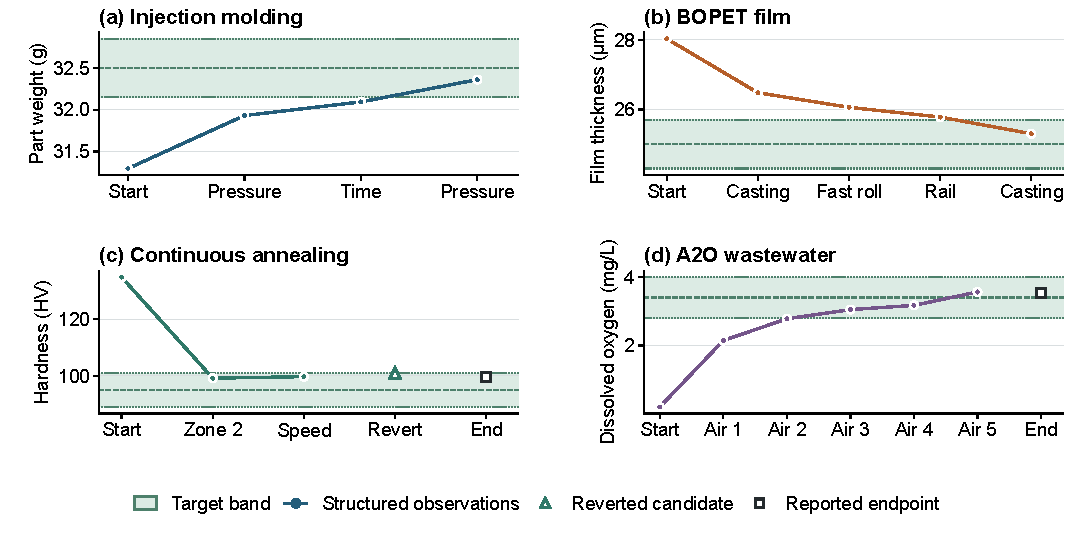
\includegraphics[width=\textwidth]{resources/fig-missions-controls.pdf}
\caption{Process observations from four simulated missions. Shading denotes
the scenario-specific target band and circles denote structured trajectory
observations. The open triangle marks the annealing candidate that was
reverted; its value comes from event text rather than a structured trajectory
record. Open squares show separately reported mission-final values for
annealing and wastewater; these are not connected to the preceding
observations. Horizontal positions indicate event order, not elapsed time.
Each panel represents one deterministic trajectory.}
\label{fig:missions}
\end{figure*}

\subsection{Injection Molding and Film Thickness}
The injection-molding mission sought a part weight of
$32.5\pm0.35$\,g. Starting at 31.296\,g, the routine requested an increase in
holding pressure from 45 to 57.73\,bar, then an increase in holding time from
6 to 10.56\,s. The corresponding observations rose to 31.93 and
32.09\,g. A further pressure request to 62\,bar preceded the final
32.36\,g observation, inside the target band. The record therefore shows
three linked adjustments in one run; it does not isolate the effect of each
parameter through a controlled comparison.

The BOPET mission sought $25.0\pm0.7$\,$\mu$m film thickness. Its initial
observation was 28.03\,$\mu$m. Four requests changed casting speed, fast-roll
speed, rail width, and casting speed again. The successive observations were
26.48, 26.06, 25.78, and 25.30\,$\mu$m. Thus the final value entered the
target band after actions on three controls; the first three observations
remained above the 25.7\,$\mu$m upper limit. The reported melt-temperature
observations during the mission were 291.3--291.8\,$^{\circ}$C, within the
configured 268--300\,$^{\circ}$C window. These measurements characterize
this simulated sequence; they do not establish a general tuning rule for
film lines.

\subsection{Annealing and Wastewater Treatment}
The annealing mission combined a hardness target of $95\pm6$\,HV with a
line-speed increase. The initial hardness was 134.9\,HV. After a zone-2
temperature request from 710 to 850\,$^{\circ}$C, a structured observation
was 99.18\,HV. A speed request from 140 to 152\,m/min was followed by
99.74\,HV. A later 164\,m/min candidate was reverted; the event text reports
101.0\,HV for that candidate, at the upper boundary of the target band.
The mission summary separately reported a final hardness of 99.5\,HV and
retained speed of 152\,m/min. The latter is 8.57\% above the initial
140\,m/min setting, not a measured production-throughput gain. The rejected
candidate reached the upper boundary and failed the configured hardness
margin rule, illustrating why the sequence retained the lower request. The
record also contains a failed zone-3 read
before the zone-2 action. Final tensile-strength and surface-defect
measurements were not archived, so the record cannot establish that all
annealing quality constraints were met.

The wastewater mission first targeted dissolved oxygen (DO) at
$3.4\pm0.6$\,mg/L. Five blower-frequency increases from 26 to 34.1\,Hz
accompanied a rise from 0.194 to 3.567\,mg/L in the structured aeration
sequence. The routine then adjusted alkali and coagulant dosing for pH and
phosphorus, followed by cost-trimming actions. Recorded total-phosphorus
observations fell from 0.662 to 0.5507, 0.4607, and 0.413\,mg/L during dosing.
A later blower reduction was reverted after the recheck found insufficient
margin. The mission separately
reported final DO of 3.54\,mg/L and a change in its simulator-defined cost
index from 182.6 to 180.2. This index is not a measured operating cost. The
complete final effluent vector was not archived; therefore the reported DO
value and cost index do not independently verify all discharge constraints.

\subsection{Evidence Synthesis}
The reported final primary variable lies within its target band in each
mission. The recorded paths differ: molding and film production combine
several actuators, annealing retains a lower-speed setting after a reverted
candidate, and wastewater treatment moves from aeration to chemical dosing.
These examples illustrate how requests and observations can be interpreted
across different simulated objectives. The protocol exercise, onboarding
replay, entry-path checks, and mock approval test address distinct integration and control
questions; their counts are not combined with the four process trajectories.
Together they do not establish
repeatability, causal effects of individual actions, comparative performance,
human-approval effectiveness, or transfer to a physical plant.

\section{Discussion}
\label{sec:discussion}
\subsection{Interpretation}
The protocol checks and onboarding replay address different steps in device
integration. Protocol connectivity demonstrates communication with the tested
simulator endpoints, while the replay checks whether one configuration exposes
its declared acquisition and control nodes. Neither establishes that an
arbitrary device can be integrated without adaptation. The entry-path checks
show which records are available for each tested call; separate environments
and absent handler-level traces prevent a claim of route equivalence or direct
verification of a shared handler. In the separate
approval-context test, stale product and run identities reach mock writes when
the tuple comparison is removed; their rejection with the comparison enabled
therefore isolates the check's contribution within that test setup.

The four missions make the distinction between a control request and a
process outcome concrete. In the molding and film examples, several requests
precede the final in-band observation; in annealing, the record also contains
a reverted candidate. In wastewater treatment, the aeration trajectory and
the later mission summary refer to different observations. Keeping these
records distinct permits the sequence to be inspected without treating a
command as proof of a desired process response.

The missions also illustrate the role of scene-specific configuration.
Part weight, film thickness, hardness, and dissolved oxygen have different
units, target bands, and available actuators. The operation--response
structure accommodates these differences, but the trajectories do not
identify which architectural component caused an outcome. Related approaches
likewise connect industrial operations to semantic skills, equipment context,
or process validation \cite{koehle2025semanticrecipes,graul2026aas,schall2026safe}.
The present study complements those designs by describing a shared operation
path and showing recorded responses in four simulated scenes; the studies use
different tasks and do not provide a matched performance comparison.

\subsection{Scope and Limitations}
The optimization evidence comprises one deterministic simulated trajectory per scene,
without independent replicates or a matched alternative controller. It cannot
establish statistical repeatability, superiority to another platform, or the
effect of individual controls. The missions use direct-node operations and
do not test the full range of entry routes or language-model decisions
described by the architecture. Final tensile-strength and surface-defect
readings for annealing and the complete final wastewater effluent vector are
missing, limiting conclusions about secondary constraints. The process model
and simulator configuration also limit transfer to physical production.

The mission records show automated judgments, not human pre-approval. The
approval-context test uses simulated decisions and mock drivers; it tests a
software condition, not operator performance or the effectiveness of human
review \cite{parasuramanmanzey2010complacency,bainbridge1983ironies}.
Software operation restrictions are not a complete security or safety
assessment \cite{greshake2023injection,liu2024pinjection,iec62443-3-3};
independent plant protection remains necessary \cite{iec61511}. Future work
should repeat missions across initial conditions, preserve all terminal
quality measurements, compare matched controllers and entry paths, and
evaluate the system with suitable physical equipment and operator oversight.

These results separate three integration decisions: which entry a caller uses,
which scene mapping an operation resolves, and which evidence an owning service
retains. This separation lets an application change an agent engine or a device
mapping without redefining the operation record. The evidence supports this as
a software structure; it does not measure engineering effort, operating cost,
or reliability gains, which would require matched deployments.

\section{Conclusion}
\label{sec:conclusion}
AgentWorkShop connects industrial task context and scene-specific device
operations through shared dispatch, configured drivers, and separately
retained command and observation records. Simulator connectivity and one
onboarding replay exercise configured protocol and node access; separate
entry-path checks record route-specific evidence, and a mock test checks stale
approval-context rejection. Four local simulation missions
illustrate the operation--response sequence across different process
objectives; their reported final primary values lie within their respective
target bands. The examples show how process evidence can be interpreted
alongside requested actions, while the single deterministic trajectories and
missing secondary measurements leave repeatability, comparative benefit,
human-review effectiveness, and physical-plant performance for future
evaluation.

\noindent\textbf{Data Availability:} Supplementary File~S1 contains the route and
integration-check records, the onboarding replay log, the archived mission
traces, and hash manifests. The manuscript source, vector figures, and
figure-source data accompany the submission package. No physical-plant data
are included.


% Start the bibliography on a fresh page and balance its two columns.
\clearpage
\balance
\bibliographystyle{IEEEtran}
% Keep IEEEtran's default bibliography size and leading.
\bibliography{resources/refs}

\end{document}
